\documentclass[Dissertation.tex]{subfiles}
\begin{document}
\chapter{Methodology}\label{chap:method}
\section{Introduction}\label{sec:methInt}
This chapter describes methodology used to develop the models that form part of the project. Throughout the project at each stage the starting point was to build a functional `baseline'. With a basic working system in place, improved iterations were then developed until performance criteria were met.

Three main model types were employed to perform stance detection in accordance with project aims. These are:
\begin{enumerate}
	\item Logistic Regression 
	\item Multi Layer Perceptron
	\item FastText Classifier
\end{enumerate}

Each type was programmed within a modular framework developed for this project to ensure consistency between models and ensure code re-usability. 
Several variants were trialled for each architecture that formulated the classification problem in different ways, such as using a label power set approach, a multi-label approach and a multi-task approach. The overall project architecture is shown in figure \ref{fig:modularProject}. This comprises five key building blocks:
\begin{enumerate}
	\item Data Extractor: Converts the raw input data into a tabular format machine readable by \texttt{Python} and splits this into training, validation and testing dataset. This block is common to all variants.
	\item Feature Pipeline: Maps input dataset to feature space. Two configurations are used:
	\begin{enumerate}
		\item Engineered Features: linguistic features used in logistic regression and multi layer perceptron
		\item Embeddings: Dense vector representation of words learned during training
	\end{enumerate} 
	\item Label Pipeline: Maps wide format tabular stance category annotations to numeric representation. Three configurations are used:
		\begin{enumerate}
			\item Multi-class
			\item Multi-label
			\item Multi-task 
		\end{enumerate}	
	\item Learning Algorithm: Model type used in learning process. Three models are used:
		\begin{enumerate}
			\item Logistic regression
			\item Multi-layer perceptron
			\item FastText classifier
		\end{enumerate}
	\item Evaluation Function: Wrapper for computing $ \mathrm{F_1} $ scores. Configuration determined by Label Pipeline.
\end{enumerate}

Results for each classifier are recorded and analysed in section \ref{}.

\begin{figure}
	\centering
	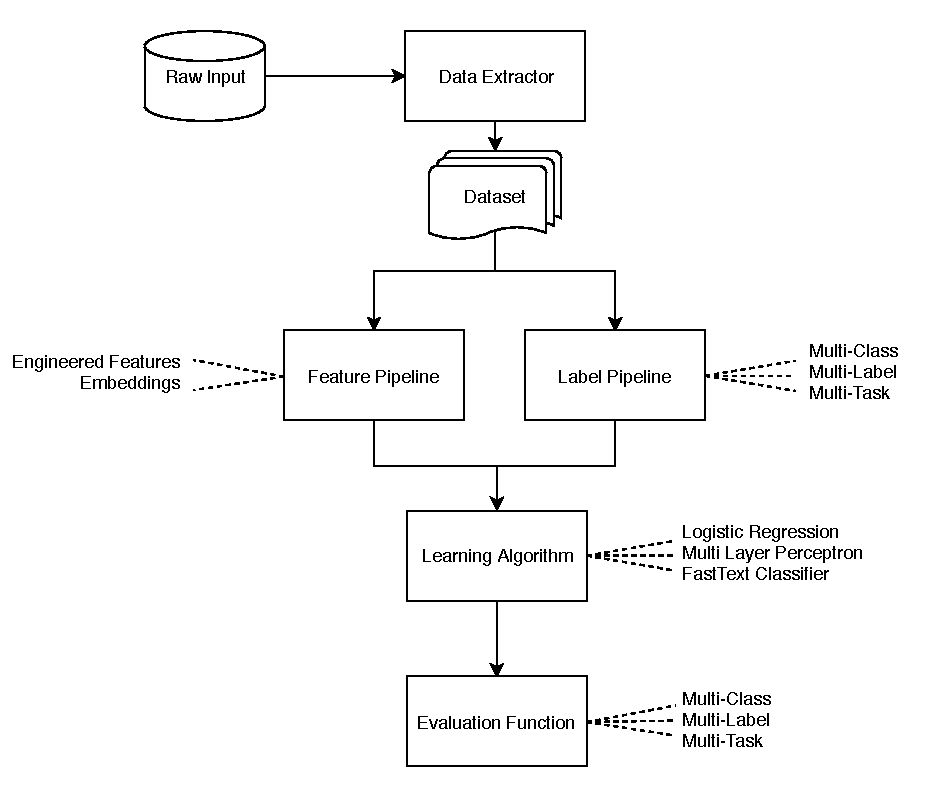
\includegraphics[width=7in]{system_architecture.pdf}
	\caption{Modular project architecture}
	\label{fig:modularProject}
\end{figure}

\section{Development Environment}
All models used in this project were written in \texttt{ Python 3.6}. Each model makes extensive used of popular data science and machine learning libraries such as \texttt{numpy, pandas} and \texttt{sklearn} (Sci-kit Learn). Neural models were developed using the \texttt{Keras} \texttt{Functional} API with a \texttt{TensorFlow} backend. Achieving high performance in short time frames using consumer technology is of interest to this project. In consideration of this, GPU acceleration is not used in any model, and all models were run on a consumer laptop with a Ubuntu operating system installed. All models complete the training and testing cycle in under ten minutes.

\section{Feature Engineering}
An important part of any machine learning task is feature selection. Bag-of-words/N-gram language models are known to perform well and generalise to many natural language processing tasks, and so these often form the starting point for feature engineering in natural language processing problems.  Consequently, an N-gram utterance representation forms part of the feature vector used in the first two model architectures.

In addition to N-gram features, count based linguistic features that encode semantic or syntactic information are commonly used in natural language processing tasks. In most cases detailed quantitative statistical analysis of such linguistic features would therefore be necessary  and form part of preliminary project research. However, in the course of the literature survey Simaki et al.\ \cite{simakiEvaluatingStanceannotatedSentences2018} was identified, which documents the results of such an analysis of the Brexit Blog Corpus. The methodology used is summarised in Section \ref{sec:quantAnalysis}.
Using one way ANOVA F-measure testing 19 linguistic features were identified that exhibited statistically significant differences in mean value across stance categories.  Since F-measure quantifies the variance of group means, it follows that linguistic features with high F-measures should be highly differentiating when included in a feature vector. Under this intuition the top ten linguistic features in \cite{simakiDetectionStanceRelatedCharacteristics2018} ranked by ANOVA F-measure (shown in Table \ref{tab:fvalue}) were used in the baseline system.

\begin{table}[h]
	\centering
	\begin{minipage}{0.6\textwidth}
		\renewcommand*\footnoterule{}
		
		
		\caption{Top 10 features by F-value}
		\label{tab:fvalue}
		\begin{tabularx}{\linewidth}{X c}
			\toprule
			Linguistic Feature 			&	F-value\\ \midrule
			Average word length			&	20.44\\
			Conjunction Frequency		& 	15.61\\
			Average sentence length (words)	& 10.60\\
			Comma frequency				&	9.42\\
			Full stop frequency			&	7.67\\
			Hapax legomena\footnote{A word which appears in a corpus only once} & 6.75\\
			Different words				&	6.63\\
			Average sentence length (characters) & 5.65\\
			Punctuation 				&	5.47\\
			Hapax dislegomena\footnote{A word which appears in a corpus only twice} & 5.50\\
			\bottomrule
		\end{tabularx}
	\end{minipage}
\end{table}

In order to build modularity and flexibility into the feature engineering process, the \texttt{Pipeline} system from \texttt{sklearn} was used. This necessitated writing custom feature extraction classes which ensured compatibility with the \texttt{Pipeline} API. A diagram of the feature extraction pipeline used is show in Figure \ref{fig:featureExtraction}. The \texttt{Sentence Feature} extractor class calculates all features in Table \ref{tab:fvalue} requiring only a single pass through the data set. The hapax legomena and hapax dislegomena features are calculated by a separate extractor taking two passes through the data. \texttt{Count Vectorizer} is class included in \texttt{sklearn} that generates the bag-of-words representation. Finally, the three results are concatenated into one feature vector through the \texttt{Feature Union} class.
\begin{figure}
	\centering
	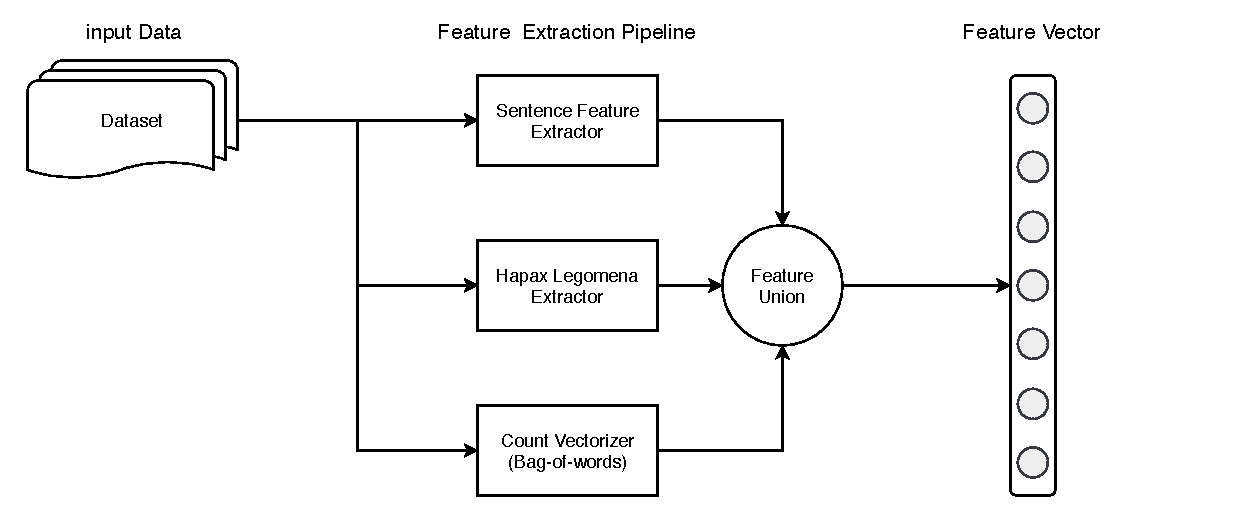
\includegraphics[width=7in]{feature_extraction.pdf}
	\caption{Feature extraction pipeline}
	\label{fig:featureExtraction}
\end{figure} 
 
\section{Label Transformations}
A key aim of this project was to investigate differences and relations between approaches to multi-label problems. Sections \ref{sec:multiLabel} and \ref{sec:multiTask} outlines how multi-label data can be transformed into multi-class (label power set) and multi-task domains. To that end, label transformation pipelines were implemented to provide consistency with the flexible, modular approach to feature extraction. The label pipeline developed provides a simple API that allows the input dataset target variable to be represented in multi-class, multi-label or multi-task formats. Figure \ref{fig:labelPipe} shows a diagram of the label pipeline. The default setting is the multi-label representation, where for each instance the target label set is represented by a one-hot encoded target vector $\mathbf{y} \in \mathcal{Y}^{10}$ where $ \mathcal{Y} = \{0,1\} $. Thus for dataset $ \mathcal{D} $ of $ N $ instances we have target variable matrix $ \mathbf{Y} \in \mathcal{Y}^{N\times10}$. The power set transformer maps the one hot encoded representation to the power set of all observed label combinations. In this representation the target label set is represented by a single index $ y \in \mathcal{Y} $ where $\mathcal{Y} = \mathcal{P}(\{0,1\}^{10})  $ with $\mathcal{P}(\{\cdot\})$ denoting power set. Therefore given dataset $ \mathcal{D} $ we have a target variable vector $ \mathbf{y} \in \mathcal{Y}^N$. Finally the multi-task transformer maps the one hot encoded  target vector to ten separate values. In this representation for each instance the target variable is a list of ten binary variables $ (y_1, y_2, \dots,y_{10} ) $ where $ \mathcal{Y} = \{0,1\} $ and $ y_i \in \mathcal{Y}$. Therefore for dataset $\mathcal{D}$ we have a list of ten target vectors, $ (\mathbf{y}_1,\mathbf{y}_2, \dots, \mathbf{y}_{10}) $ where $ \mathbf{y}_i \in \mathcal{Y}^N $. In summary, the label pipeline architecture provides a simple solution for switching between classification domains in order to compare their performance on the same dataset.
	
\begin{figure}

	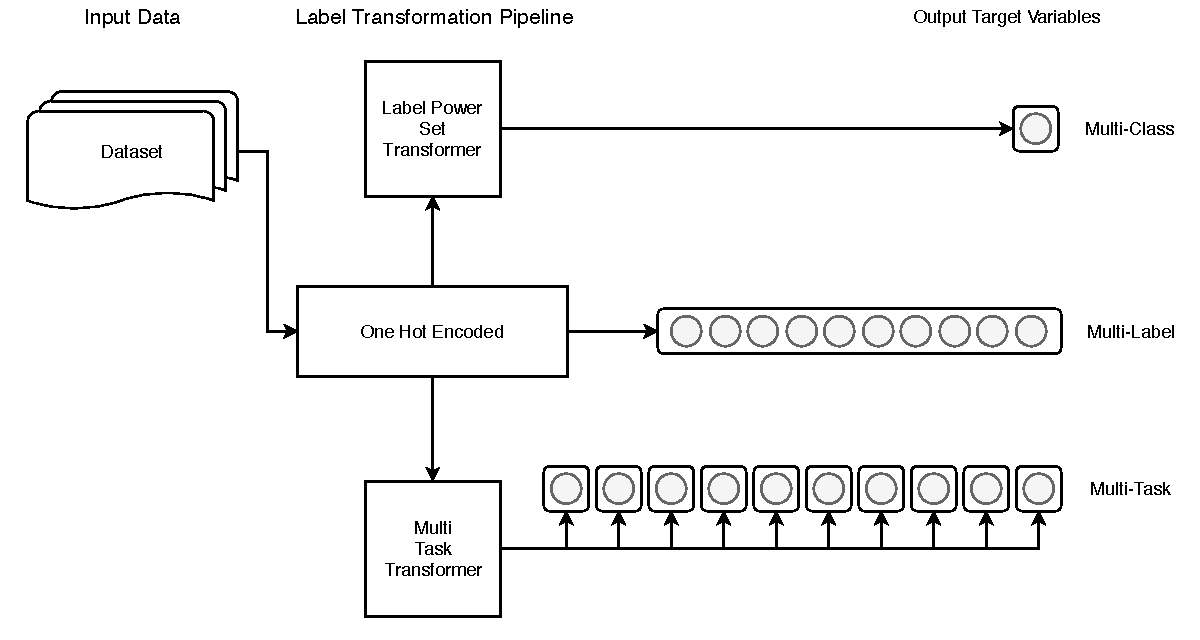
\includegraphics[width=6in]{multi_paradigms.pdf}
	\caption{Label pipeline diagram showing transformation pathway for multi-class, multi-label and multi-task target variable representations}
	\label{fig:labelPipe}
\end{figure}

\section{Output Layers}\label{sec:outputLayers}
As part of the modular architecture proposed in this project, a common set of output layer configurations was written to be used in the neural models, namely the MLP and FastText classifiers. In figure \ref{fig:outLayers} is a diagram showing the different configurations. In the multi-class configuration, the output layer contains one node for each of the stance category combinations observed from the label power set. In section \ref{sec:EDA} 92 combinations were identified in the dataset,  therefore the multiclass output layer uses 92 nodes and a softmax activation layer. The model prediction is therefore given by the class with highest probability. In the multi-label configuration, there is simply one output layer with one node per stance category (ten nodes in total), and the layer uses a sigmoid activation. Consequently, the set of stance categories predicted is given by the set of output nodes with probability $ p\geq0.5 $. In the multi-task configuration, each stance category is modelled as a separate task, so there are ten output layers, each consisting of one node with a sigmoid activation. Again, the set of stance categories is predicted is given by output nodes with probability $ p\geq0.5 $. The entire network prior to the output layers is shared between tasks.

\begin{figure}
	\centering
	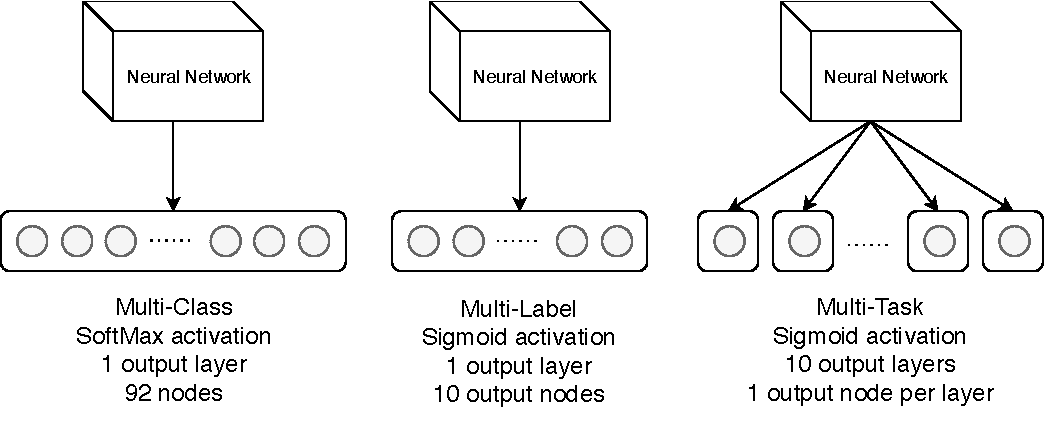
\includegraphics[width=5.5in]{out_layers.pdf}
	\caption{Output layer configuration for neural models in multi-class, multi-label and multi-task classification domains}
	\label{fig:outLayers}
\end{figure}

\section{Logistic Regression Baseline}
The first model tested was a simple logistic regression classifier using \texttt{sklearn} and default hyper-parameters. This model serves as the project baseline, and therefore a key goal for subsequent models is to improve upon the performance of the logistic regression classifiers. In accordance with project aims, logistic regression was implemented and compared in the multi-class and multi-label domains. The multi-class implementation uses the label pipeline power set transformation, and the multi-label implementation uses a binary relevance transformation of the dataset (as described in section \ref{sec:multiLabel}) by using the functional equivalent in \texttt{sklearn}, the \texttt{OneVsRestClassifier} wrapper.

\section{Multi-Layer Perceptron}

\begin{figure}
	\centering
	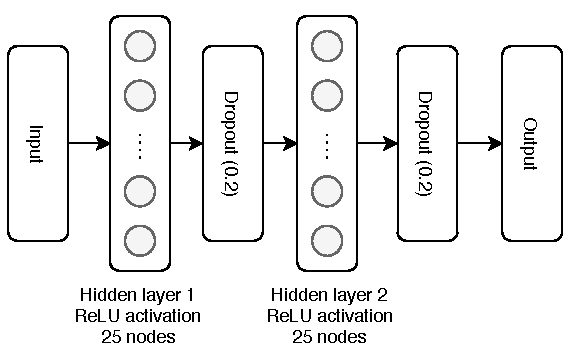
\includegraphics[width=5in]{mlp.pdf}
	\caption{Multi-layer perceptron configuration used in testing}
	\label{fig:mlp}
\end{figure}
The Multi-Layer Perceptron (MLP) is known to be a robust and versatile neural network model \cite{castellaniCompetitiveCoevolutionMultilayer2018} with applications in many machine learning tasks. The MLP was the second model tested in this project, and forms the starting point for investigation of deep learning models in this project. Figure \ref{fig:mlp} shows a diagram of the configuration used. A hidden layer size of 25 nodes per layer provided an optimal balance between performance and computational cost, and drop out layers were included as a regularisation measure to improve generalisation of the model. Using the architecture described in Section \ref{sec:methInt} the MLP was implemented in multi-class, multi-label and multi-task formats. Section \ref{sec:outputLayers} describes in detail the differences between output layers across classification domains.

\section{FastText Classifier}\label{sec:fastTextMethod}
The third model implemented is the FastText classifier. FastText is know to be a very efficient, high performance architecture for learning embeddings and text classification that offers similar accuracy to recurrent networks and convolutional  networks at a much lower computational cost \cite{joulinBagTricksEfficient2016}. It is therefore very suitable for this project given the aim to research high performance deep learning methods that do not require GPU acceleration or other specialised hardware. Figure \ref{fig:fastTextClassifier} shows the configuration used. Each word in the input is mapped to a vector of length 100 in the embedding layer, and the average pooling layer takes the mean of all embeddings in the embedding layer. The embedding layer therefore learns an embedding for each word in the dataset vocabulary during training, and weights are learned between the average pooling layer and the output layer. FastText classifier was implemented in multi-class, multi-label and multi-task formats, again using the architecture described in Section \ref{sec:methInt} and Section \ref{sec:outputLayers}.

\begin{figure}\centering
	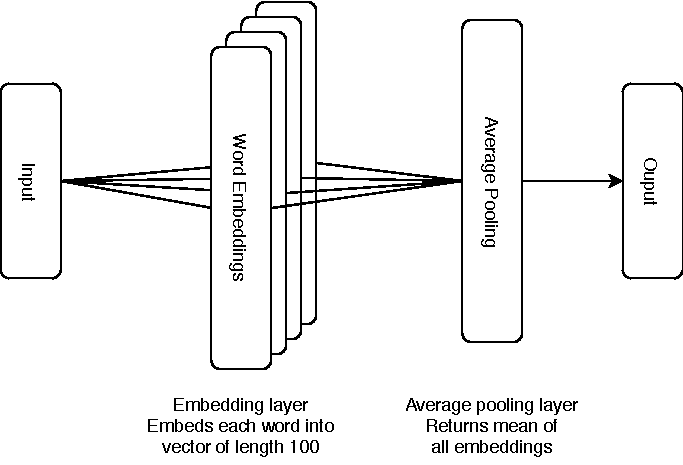
\includegraphics[width=5in]{fast_text_classifier.pdf}
	\caption{FastText classifier configuration used in testing}
	\label{fig:fastTextClassifier}
\end{figure}





\end{document}